\documentclass[paper=a4,
	fontsize=10pt,
	DIV=18,
	twocolumn,
	parskip=half
	]{scrartcl}
\usepackage[font=small,labelfont=bf,format=plain,margin=10pt]{caption}
\usepackage{bijan_koma}
\usepackage[ngerman]{babel} 


%%%%%%%%%%%%%%%%%%%%%% Settings for packages %%%%%%%%%%%%%%%%%%%%%%%%%%%%%%%%%%

\usepackage[range-phrase={\,\,bis\,\,}]{siunitx}  % Correct typesetting of units
\sisetup{       
  separate-uncertainty,
  per-mode=fraction
}

\colorlet{darkblue}{blue!70!black}
\hypersetup{
  colorlinks,
  citecolor=darkblue,
  filecolor=darkblue,
  linkcolor=darkblue,
  urlcolor=black
}

\crefformat{equation}{Glg.~(#2#1#3)}
\crefformat{section}{Abschnitt~#2#1#3}
\crefformat{figure}{Abb.~#2#1#3}
\crefformat{table}{Tab.~#2#1#3}
\crefformat{chapter}{Kapitel~#2#1#3}


\addto\captionsngerman{             % Changes Abbildung->Abb.,etc. in caption 
  \renewcommand{\figurename}{Abb.}
  \renewcommand{\tablename}{Tab.}
}

\numberwithin{equation}{section}    % Number equations after sections, e.g. (1.2)

%%%%%%%%%%%%%%%%%%%%%% Headings and seperation lines %%%%%%%%%%%%%%%%%%%%%%%%%%

\usepackage[automark,markuppercase]{scrpage2}     % AUTOMATIC HEADINGS
\pagestyle{scrheadings}                           % Apply userdefined settings
\setheadsepline{.5 pt}                            % Width of seperation line
\setkomafont{pagehead}{\normalfont}               % Use normalfont for heading
\cfoot{\thepage}                                  % Page numbering 

%%%%%%%%%%%%%%%%%%%%%% Spacings %%%%%%%%%%%%%%%%%%%%%%%%%%%%%%%%%%%%%%%%%%%%%%%

\columnsep20pt                                  % Width inbetween \twocolumns
%\onehalfspacing                                 % 1.5 line spacing
\linespread{1.2}

\setlength{\headheight}{2.0\baselineskip}       % Fixes the 'small headhight'

\renewcommand*{\chapterheadstartvskip}{\vspace{0\baselineskip}} 
% Spacing Pagehead-Headline. Standard: 2

\renewcommand*{\chapterheadendvskip}{\vspace{\baselineskip}}
% Spacing Headline-Text

% Spacing in math environments \,\;.. 
%\thinmuskip=3mu % default
%\medmuskip=4mu plus 2mu minus 4mu % default is 4 mu p2 m4
%\thickmuskip=5mu plus 5mu % default

\allowdisplaybreaks[1]  % optional argument denoting permissiveness of page breaks 
% in equations. 1 ="allow page breaks but avoid them" and 4="break whenever you want".

\newcommand{\tra}{$\rightarrow $}
\newcommand{\Tra}{$\Rightarrow $}
\renewcommand{\note}[1]{{\color{red}#1??}}

\usepackage{url}
\usepackage[numbers]{natbib}
\usepackage{textcomp}


\usepackage{paralist}

\newcommand{\kor}[1]{{\color{green}#1}}
%%%%%%%%%%%%%%%%%%%%%%%%%%%%%%%%%%%%%%%%%%%%%%%%%%%%%%%%%%%%%%%%%%%%%%%%%%%%%%%%
%ToDo:

%%%%%%%%%%%%%%%%%%%%%%%%%%%%%%%%%%%%%%%%%%%%%%%%%%%%%%%%%%%%%%%%%%%%%%%%%%%%%%%%

\begin{document}

\title{Kernspinresonanz}                  
\author{Daniel Friedrich \& Ulrich Müller}         
\date{}                                % Turn off automatic date
\twocolumn[\begin{@twocolumnfalse}
\vspace{-3em}
\maketitle      
%=============================================================================
\begin{abstract}      
%=============================================================================
  \vspace{-2em}
  \noindent {\small 
  	Ein Wasserkreislauf, Polarisator, Manipulator und Analysator ergeben einen Aufbau zur Untersuchung der magnetischen Kernresonanz. Wir bestimmen die Resonanzfrequenz $\nu_{\rm res} = \SI{4712.31}{\kilo\hertz}$ der Protonen im Feld des Analysators sowie die Energieaufspaltung $\Delta E = \SI{19.48854e-9}{\electronvolt}$. Wir stellen den Phasenraum von Frequenz, Amplitude und Signal dar, nehmen 4 volle Drehungen des Spins auf und bestimmen das Kernmagneton $\mu_{\rm K} = \SI[per-mode=symbol]{5.0979e-27}{\tesla\per\ampere}$. Wir bestimmen das vorhandene Störfeld im Raum und vergleichen für verschiedene Temperaturen die Relaxationszeiten $T_1$, wobei wir bei höherer Temperatur längere Relaxationszeit messen. Insgesamt konnten wir die theoretisch vorhergesagte Dynamik der Magnetisierung bestätigt.
    }
\end{abstract}

  \vspace{1em}

\centerline{Betreuer: Dr. Charles Gould \hfill
   Versuchsdurchführung am 18. Oktober 2013}
\centerline{\hfill  Protokollabgabe am 25. Oktober 2013}
 

\vspace{2em}
%
\end{@twocolumnfalse}
]
%
% =============================================================================
\section{Einleitung}
\label{Einleitung}
%
Befindet sich ein Atomkern mit einem nichtverschwindem Spin in einem Magnetfeld, so kann er elektromagnetische Strahlung absorbieren sowie emittieren. Dieser Effekt wird als Kernspinresonanz (eng.: nuclear magnetic resonanz NMR) bezeichnet.
Zurückzuführen ist der Effekt auf das magnetische Moment, das durch den Spin des Atomkerns hervorgerufen wird. Dieses magnetische Moment besitzt, je nach Orientierung in einem äußeren Magnetfeld, unterschiedlich viel Energie. 
Die Energieaufspaltung eines Spins im äußeren Magnetfeld wurde zuerst im Jahre 1896 von Pieter Zeeman an Elektronen in einem Atom und 40 Jahre später von Isidor Rabi an Atomkernen nachgewiesen~\citep{rabi}.\\
Kleinste Unterschiede im lokalen magnetischen Feld von Atomkernen werden in der Chemie eingesetzt um Informationen über den Bindungszustand von Atomen zu gewinnen. Die Unterscheidung von Materialien aufgrund der Kernspinresonanz ermöglicht in der Magnetresonanztomographie zerstörungsfrei Bilder von organischen Proben in Echtzeit aufzunehmen~\citep{nmr}.


%
% =============================================================================
\section{Theorie}
\label{Theorie}
%
\label{theorie}
Die Theorie der Kernspinresonanz ist auf die Wechselwirkung zwischen dem magnetischen Moment des Atomkerns und dem äußeren Magnetfeld zurück zu führen.
Das magnetische Moment des Kerns wird dabei von dessen Spin verursacht und folgt der Beziehung
\begin{align}
\vec{\mu}=g \frac{\mu_{\rm K}}{\hbar}\vec{s}
\end{align}
mit $g$ dem Landé-Faktor des Protons, $\hbar$ dem planck'schen Wirkungsquantum und $\mu_K$ dem Kernmagneton. Für ein Proton entspricht dabei das Kernmagneton äquivalent zum Bohrschen Magneton $\mu_{\rm K}=\frac{e \hbar}{2m_{\rm p}}$ mit $m_{\rm p}$ der Protonenmasse. Der Landé-Faktor des Protons beträgt etwa 5.59.\\
Befindet sich das magnetische Moment nun in einem Magnetfeld, so besitzt es die potentielle Energie 
\begin{align}
E_{\rm M}=-\vec{\mu} \cdot \vec{B}
\end{align}
und ist somit in seiner energetisch günstigsten Position, wenn es parallel zum äußeren Feld ausgerichtet ist.

In einer Probe kommt ein großes Ensemble von Protenenspins vor, sodass sich die Gesamtmagnetisierung $\vec{M}$ der Probe aus der Summe der Erwartungswerte aller magnetischen Momente ergibt~\citep{anleitung}.
\begin{equation}
	\vec{M} = \underset{k=1}{\overset{N}{\sum}} \braketop{\psi_k}{\hat{\vec{\mu}}}{\psi_k}
\end{equation}
$\ket{\psi_k}$ beschreibt hier die Zustandsfunktionen der $N$ Protonen.

Jedes geladene Teilchen mit Drehimpuls $\vec{J}$ besitzt einen magnetischen Dipol $\vec{\mu}$, wodurch in einem Magnetfeld $\vec{B}$ ein Drehmoment $\vec{D}$ auf das Teilchen wirkt. Hierdurch beginnt der Drehimpuls des Teilchens um das angelegte Magnetfeld mit $\vec{D} = \vec{\mu} \times \vec{B}$ zu präzedieren. Die Präzessionsbewegung kann nach~\citet{anleitung} ?? durch
\begin{equation}
	\mathrm{d}\vec{D}(t) = \gamma\vec{M}(t) \times \vec{B}(t)\,\mathrm{d}t
\end{equation}
beschrieben werden, wobei $\gamma$ dem gyromagnetischen Verhältnis entspricht, durch das ebenso die Richtung und Größe des Dipols mit $\vec{\mu} = \gamma\vec{J}$ definiert ist.
Die Frequenz der Präzession wird Larmorfrequenz $\omega_{\rm Larmor}$ genannt und ist gegeben durch~\citep{mueller}
\begin{equation}
	\omega_{\rm Larmor} = \frac{g \mu_{\rm K}}{\hbar}B = \gamma \cdot B.
\end{equation}

Um nun die dynamische makroskopische Magnetisierung der Probe zu beschreiben werden die sogenannten Bloch-Gleichungen verwendet~\citep{anleitung}.
\begin{equation}
	\frac{\mathrm{d}\vec{M}}{\mathrm{d}t} = \gamma\vec{M} \times \vec{B}(t) - \vec{e}_x \frac{M_x}{T_2} - \vec{e}_y \frac{M_y}{T_2} - \vec{e}_z \frac{M_z}{T_1}
	\label{bloch}
\end{equation}
$T_{1,2}$ sind hier Relaxationszeiten, wobei $T_{1}$ der Zeit entspricht, mit der sich die Spintemperatur an die Temperatur des Gesamtsystems angleicht ($z$-Richtung) und $T_2$ der Zeit, in der die Spins in $x$-$y$-Richtung dephasieren.

Im Experiment befindet sich die Probe in einem statischen Magnetfeld $B_0$, wodurch eine Präzession mit der Larmorfrequenz um die Magnetfeldachse zustande kommt. Wird nun ein zusätzliches zirkular polarisiertes Feld $B_1$ eingestrahlt, kann der Drehwinkel der Präzessionsbewegung verändert werden. Das zirkulare Feld $B_1$ wird mit der selben Frequenz wie die Präzessionsfrequenz der Teilchen eingestrahlt. Hierdurch wirkt im Bezugssystems des Spins ein konstantes Magnetfeld, welches die Präzessionsbewegung des Drehimpulses neu ausrichtet. Die nötige Frequenz das zirkularen Feldes $B_1$ wird durch die Resonanzfrequenz $\nu_{\rm res}$ beschrieben~\citep{anleitung},
\begin{equation}
	\nu_{\rm res} = \frac{\gamma B_0}{2\pi}
\end{equation}
und entspricht genau der Larmorfrequenz der Präzessionsbewegung der Teilchen.

Befinden sich die Protonen nicht dauerhaft im zirkularen polarisiertem Magnetfeld, so kann erreicht werden, dass sich die Magnetisierung nur um einen gewissen Winkel, den Drehwinkel $\Phi$, dreht. So kann erreicht werden, dass sich die Magnetisierung von der $z$-Achse zum Beispiel in die $x$-Achse dreht. Der Drehwinkel ergibt sich aus dem gyromagnetischen Verhältnis $\gamma$, der Magnetfeldstärke $B_1$ und der Zeit $t_\mathrm{Spule}$ in der sich die Protonen im Magnetfeld befinden
\begin{align}
	\Phi=\gamma B_1 t_\mathrm{Spule}.
\end{align}
In der Realität kämpft man mit zwei Herausforderungen: Erstens entspricht die Anregungsfrequenz oft nicht der Frequenz, mit der die Protonen um die $z$-Achse präzedieren und zum andern ist die Zeit $t_\mathrm{Spule}$ aufgrund unterschiedlicher Geschwindigkeiten der Protonen nicht identisch. Die Abweichung der Anregungsfrequenz kann zumindest für unendlich große Relaxationszeiten analytisch gelöst werden. Die normierte $z$-Komponente der Magnetisierung ergibt sich dabei zu
\begin{align}
	\frac{M_z(\Phi, \nu)}{M(t=0)}=\frac{\left[ u(\nu)^2+\cos(\Phi)\sqrt{1+u(\nu)^2} \right]}{1+u(\nu)^2},
\end{align}
wobei $u(\nu)$ die Abweichung von der Resonanzfrequenz berücksichtigt.
Die unterschiedliche Verweildauer der Protonen in der Spule kann bei turbulenter Strömung mit einer Gaußverteilung des Drehwinkels berücksichtigt werden. 
%
% =============================================================================
\section{Experimenteller Aufbau}
\label{Experiment}
% =============================================================================
%
Der verwendete Versuchsaufbau ist in Abbildung~\ref{fig.versuchsaufbau} schematisch dargestellt.

\begin{figure}[htp]
	\begin{center}
		\includegraphics[width=\columnwidth]{Bilder/nmr_aufbau}
		\caption{Schematischer Versuchsaufbau nach~\citet{anleitung}.}
		\label{fig.versuchsaufbau}
	\end{center}
\end{figure}

Das für die Magnetisierung verwendete destillierte Wasser wird von einer Pumpe  mit einstellbarer Geschwindigkeit durch einen Wasserkreislauf gepumpt.
Als erstes wird das Wasser durch einen Polarisationsmagneten befördert. Im Magneten durchläuft es ein Labyrinth mit dem die Verweildauer erhöht wurde um eine ausreichende Polarisierung zu erzeugen.
Das polarisierte Wasser durchläuft dann ein Hemholtzspulenpaar mit dem ein statisches Magnetfeld erzeugt werden kann. Im Zentrum der Spulen ist der Wasserschlauch von einer Einstrahlspule umwickelt, die über ein Funktionsgenerator mit \SI{50}{\ohm} Output, ein Wechselfeld erzeugen kann. Mit dem Wechselfeld kann im Versuch die Richtung der Magnetisierung manipuliert werden. Der Teil wird somit auch Manipulator genannt.
Aus dem Manipulator wird das Wasser in den Analysator gepumpt, in dem die $z$-Komponente der Magnetisierung gemessen werden kann. Der Analysator besteht aus einem Hufeisenmagneten, der ein konstantes Magnetfeld erzeugt. Der Hufeisenmagnet ist zudem mit einer Spule umwickelt an die ein Wechselfeld mit \SI{50}{\hertz}, das sogenannte Wobbelfeld, angelegt wird. Somit können wir ein sich zeitlich langsam änderndes Magnetfeld erzeugen, das zu jedem Zeitpunkt für die Magnetisierung als statisch angesehen werden kann. Um den Schlauch im Inneren des Hufeisenmagneten ist eine weitere Spule gewickelt, die mit einem Schwingkreis verbunden ist, dessen Frequenz des Wechselfeldes einstellbar ist.
Nach dem Analysator gelangt das Wasser zurück in einem Sammelbehälter indem durch eine lange Verweilzeit das Wasser vollständig depolarisieren kann. Der Sammelbehälter schließt letztendlich den Wasserkreislauf.

Durch den Aufbau des Analysators kann die Frequenz des Regelkreises ebenso auf Resonanzfrequenz eingestellt werden, wodurch Übergänge zwischen den Energieniveaus der Protonen angeregt werden. Dieser Übergang absorbiert oder überträgt Leistung auf den Schwingkreis. Der Schwingkreis wird automatisch nachgeregelt. Aus diesem Leistungsausgleich entsteht unser Messsignal.
Das Signal des Analysators kann über einen Sample/Hold Verstärker (S/H-Verstärker) mit dem Oszillographen verbunden und mit dem Computer ausgelesen werden.
Der S/H-Verstärker wird durch die selbe Sinusspannung getriggert, die das Wobbelfeld erzeugt. Der Verstärker misst zu jedem Triggerimpuls kurz das Messsignal und gibt es bis zum nächsten Impuls als Gleichspannung aus. So kann durch richtige Einstellung der Phase die Höhe der Resonanzpeaks ausgelesen werden.

Die gesamte Beschaltung des Messaufbaus ist in Abbildung~\ref{fig.beschaltung} gezeigt. Im Versuch wurden allerdings nur für den jeweiligen Versuchsteil wichtige Geräte miteinander verschaltet.

\begin{figure}[htp]
	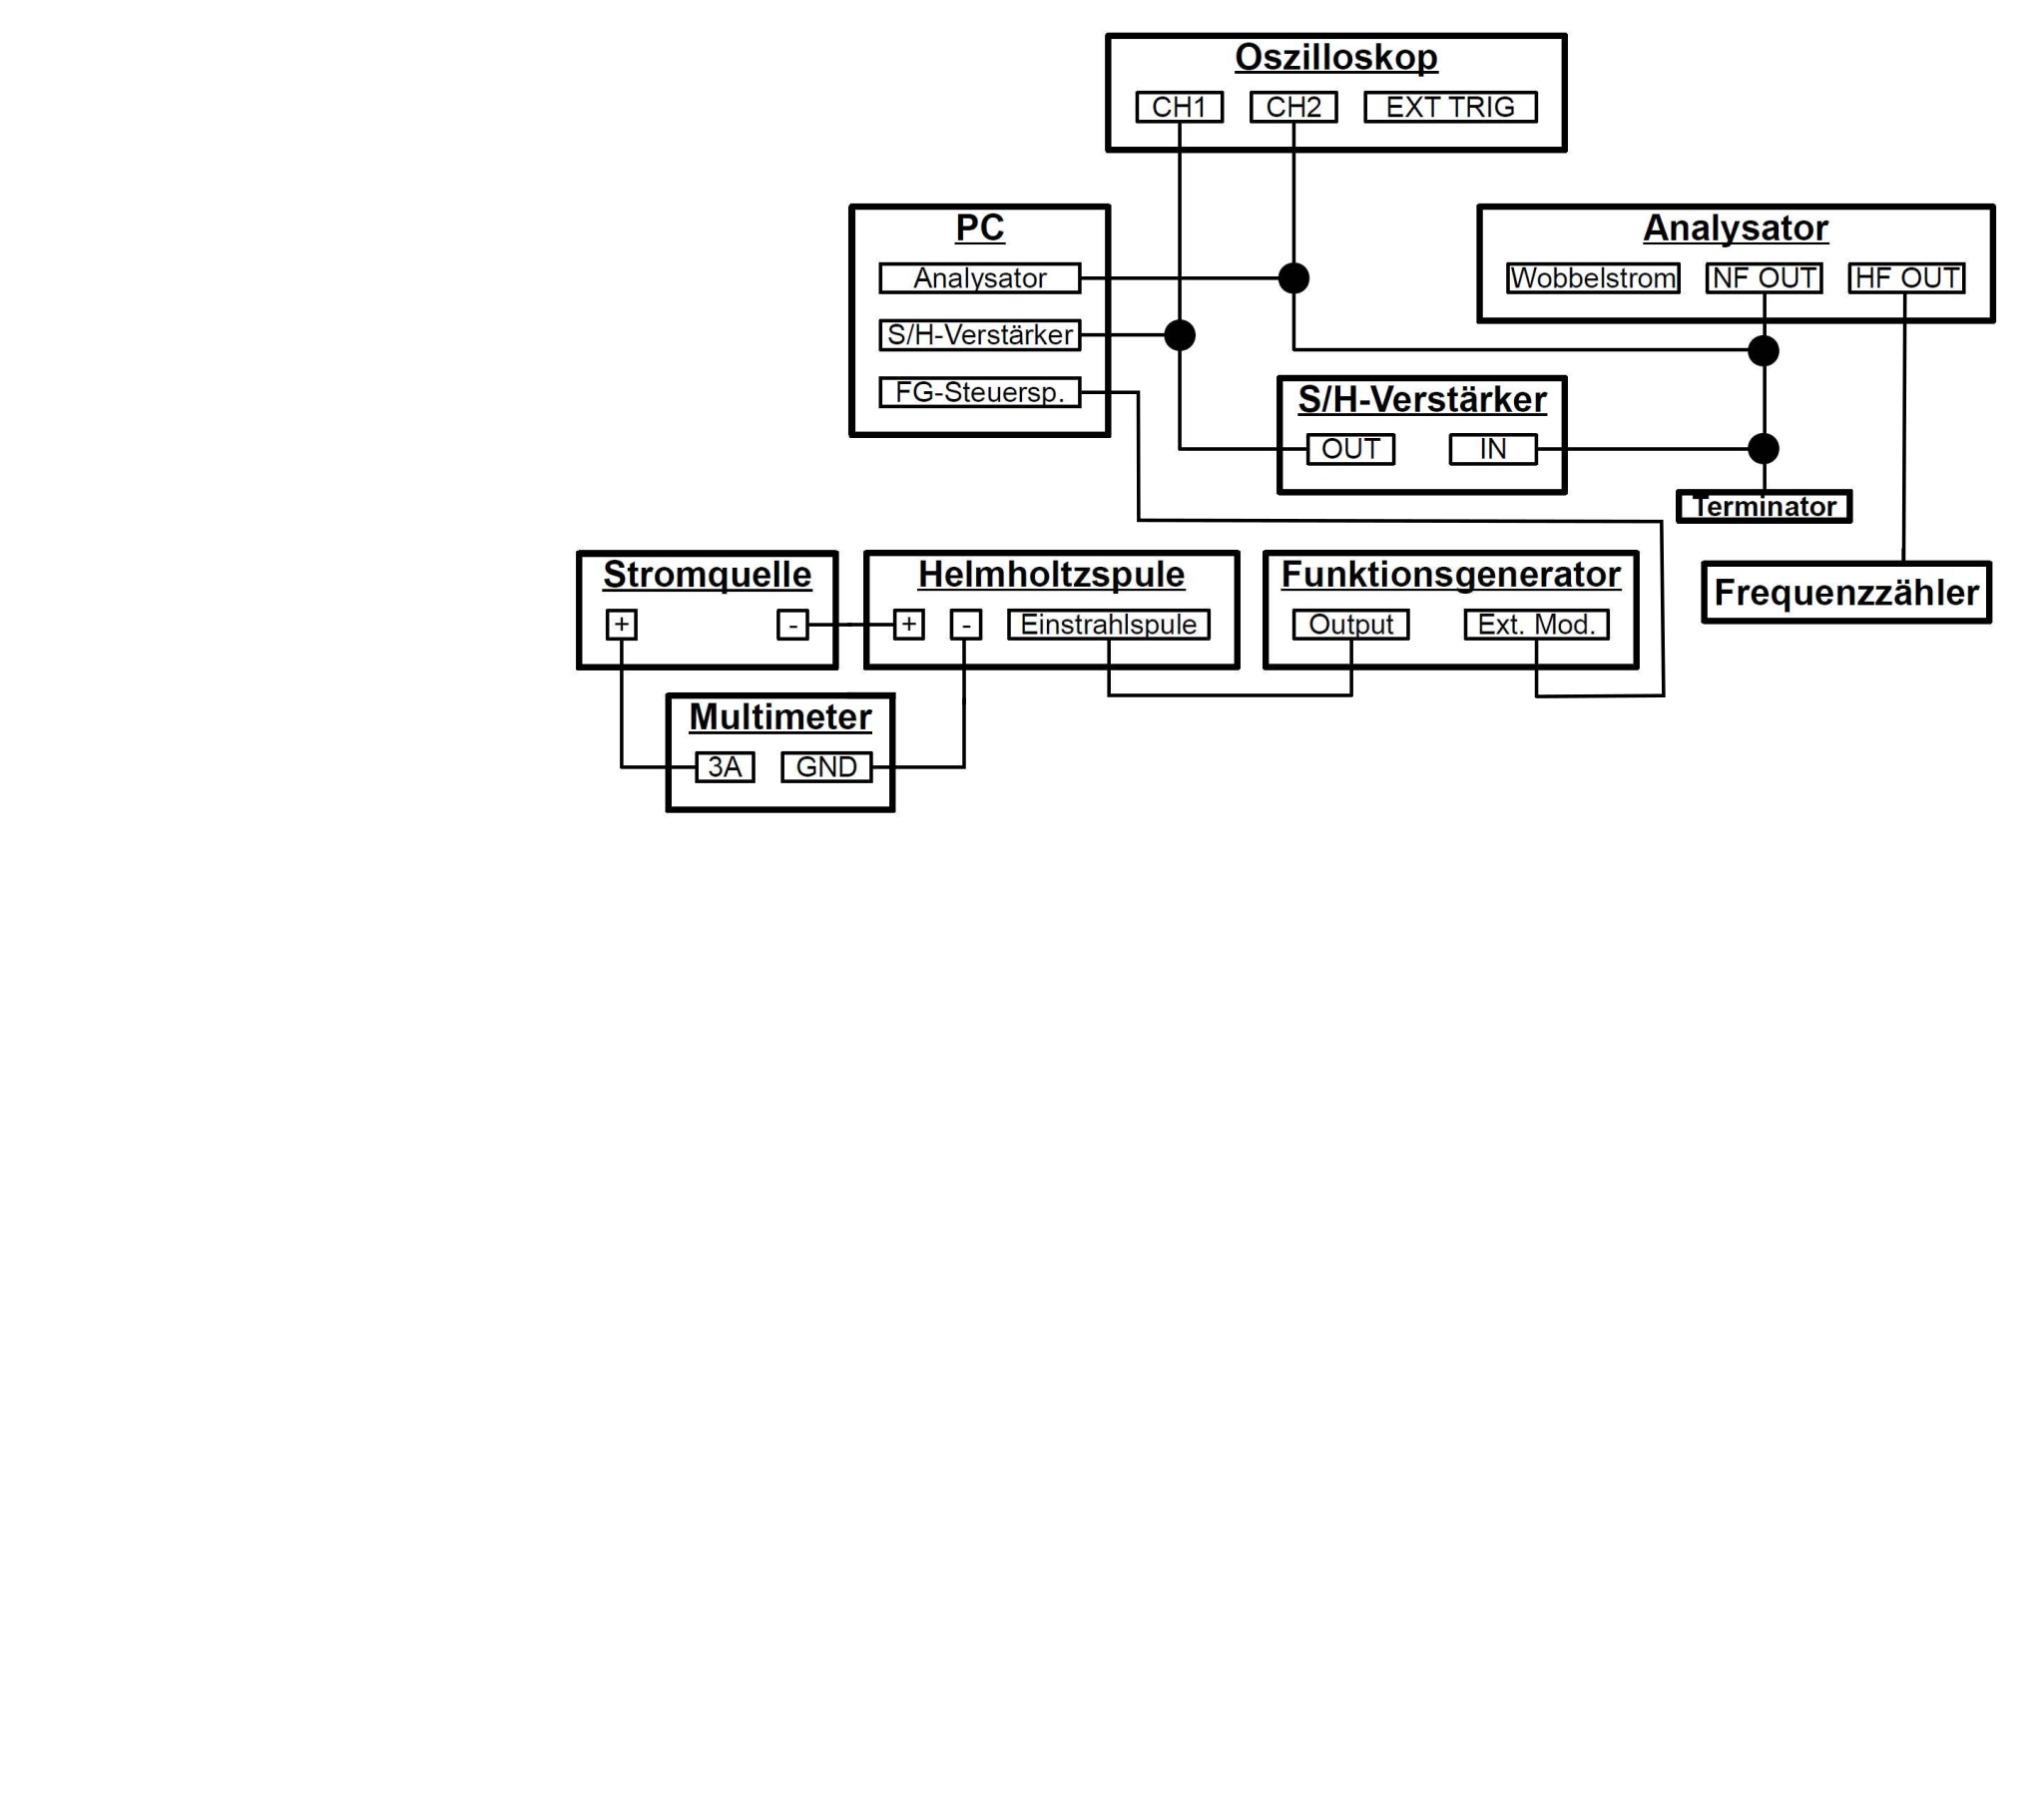
\includegraphics[width=\columnwidth]{Bilder/messbeschaltung.pdf}
	\caption{Beschaltung des gesamten Messaufbaus. Auszüge aus~\citet{anleitung}.}
	\label{fig.beschaltung}
\end{figure}

%
% =============================================================================
\section{Auswertung}
\label{auswertung}
% =============================================================================
%
% ~~~~~~~~~~~~~~~~~~~~~~~~~~~~~~~~~~~~~~~~~~~~~~~~~~~~~~~~~~~~~~~~~~~~~~~~~~~~~
\subsection{Eichen des Funktionsgenerators}
\label{auswertung1}

Um die ?? Genauigkeit des Funktionsgenerators zu überprüfen, wird dieser mit dem Oszillographen verbunden. Mit den eingestellten Werten von \SI{50}{\milli\volt} bzw. \SI{100}{\milli\volt} in der Amplitude und \SI{1.3}{\kilo\hertz} bzw. \SI{2.6}{\kilo\hertz} in der Frequenz des Funktionsgenerators messen wir das Cosinus-Signal über den Oszillator, der für die Aufnahme mit dem Computer verbunden ist. An die erhaltenen Messsignale fitten wir jeweils eine Cosinus-Funktion um die Schwankung, die durch die diskrete Zeitauflösung zustande kommt, auszugleichen. Der Fehler der Werte ergibt sich aus der Ungenauigkeit in der Amplitude des Funktionsgenerators von \SI{2}{\percent}. Der Fehler der Fitfunktion kann gegen den Fehler in der Amplitude vernachlässigt werden. Für die vier Messungen vergleichen wir jeweils die Spitze/Spitze Werte, die Amplituden und den Effektivwert. Die Werte sind in Tabelle~\ref{tab.funktionsgenerator} aufgelistet.

\begin{table}[htp]
\begin{center}
	\begin{tabular}{c|ccc}
		\hline
		\multicolumn{1}{c|}{FG \SI{50}{\milli\volt}} &\multicolumn{3}{c}{Oszillograph Spannung in \SI{}{\milli\volt}}\\
\footnotesize Frequenz & \footnotesize Amplitude & \footnotesize Spitze/Spitze & \footnotesize Effektivwert\\
		\hline
		 \SI{1.3}{\kilo\hertz} & \SI{50.2(10)}{} & \SI{100.6(20)}{} & \SI{35.55(71)}{}\\
		 \SI{2.6}{\kilo\hertz} & \SI{49.9(10)}{} & \SI{99.9(20)}{} & \SI{35.31(71)}{}\\
		 \hline
		\multicolumn{1}{c|}{FG \SI{100}{\milli\volt}} && \\
		 \SI{1.3}{\kilo\hertz} & \SI{100.2(20)}{} & \SI{200.2(40)}{} & \SI{70.87(14)}{}\\
		 \SI{2.6}{\kilo\hertz} & \SI{100.3(20)}{} & \SI{200.6(40)}{} & \SI{70.93(14)}{}\\
		\hline
	\end{tabular}
	\caption{Vergleich der eingestellten Werte am Funktionsgenerator (FG) mit den am Oszilloskop gemessen Daten, sowie die gemessenen Spitze/Spitze Werte, die Amplituden und Effektivwerten.}
	\label{tab.funktionsgenerator}
\end{center}
\end{table}

Aus dem Vergleich der Werte in Tabelle~\ref{tab.funktionsgenerator} ergibt sich im Rahmen der Fehler kein Unterschied zwischen den Werten am Oszillographen und den eingestellten Werten. Anhand der berechneten Werte erkennt man, dass die Genauigkeit des Funktionsgenerators auch bei unterschiedlichen Amplituden und Frequenzen erhalten bleibt.

Die Einstrahlspule im Manipulator besitzt einen vernachlässigbar kleinen Innenwiderstand. Allerdings ist der Spule um, den Strom zu begrenzen und messbar zu machen ein Vorwiderstand von \SI{47}{\ohm} eingebaut~\citep{anleitung}. Aus dem zusätzlichen Ausgangswiderstand des Funktionsgenerator von \SI{50}{\ohm} wird die Amplitude der Ausgangsspannung reduziert~\citep{anleitung}. Um für nachfolgende Messungen einen Eichfaktor $E_{\rm Spule}$ zu erhalten haben wir obige Messung für eine Frequenz von \SI{1.3}{\kilo\hertz} und die Amplituden \SI{10}{\milli\volt}, \SI{20}{\milli\volt}, \SI{50}{\milli\volt}, \SI{100}{\milli\volt}, \SI{200}{\milli\volt} und \SI{500}{\milli\volt} wiederholt. Hierbei haben wir jeweils eine Messung mit und eine ohne angeschlossener Einstrahlspule aufgenommen. Zur Bestimmung des Eichfaktors $f_{\rm ES}$ haben wir in Abbildung~\ref{fig.eichfaktor} die gemessenen Spannungen mit angeschlossener Spule $U_{\rm ES}$ über die eingestellten Spannungen des Funktionsgenerators $U_{\rm FG}$ aufgetragen.

\begin{figure}[htp]
	\includegraphics[width=\columnwidth]{Data-Plots/03-Effektivwert-es-fg.pdf}
	\caption{Gemessene Spulenspannung an der Einstrahlspule $U_{\rm ES}$ über die eingestellte Spannung am Funktionsgenerators $E_{\rm FG}$ zur Bestimmung des Eichfaktors.}
	\label{fig.eichfaktor}
\end{figure}

Die Werte in Abbildung~\ref{fig.eichfaktor} sind mit den entsprechenden Fehlern in der Amplitude des Funktionsgenerators (\SI{2}{\percent}) aufgetragen. Zur Bestimmung der Steigung haben wir eine ausgleichende Gerade mit Fehlergeraden an die Daten gelegt. Die Fehler des Fits können vernachlässigt werden.
Für den gemessenen Eichfaktor ergibt sich somit ??
\begin{equation}
	f_{\rm ES} = \frac{U_{\rm ES}}{U_{\rm FG}} = \SI{0.4839(97)}{}
\end{equation}
Aus den gemessen Werten erkennen wir, dass der Eichfaktor unabhängig von der gemessenen Frequenz der Wechselspannung an der Einstrahlspule ist. Dies ist auch wichtig um den Eichfaktor für spätere Versuche verwenden zu können, da dort an unterschiedlichen Frequenzen gemessen wird.

Der Eichfaktor kann zudem theoretisch aus der Kenntnis der Widerstandswerte bestimmt werden. 
\begin{equation}
	f_{\rm ES} = \frac{R_{\rm ES}}{R_{\rm FG}+R_{\rm ES}} = \SI{0.4845(97)}{}
\end{equation}
Der Fehler ergibt sich aus dem geschätzten Fehler des Vorwiderstandes von \SI{2}{\percent}.

Aus dem Vergleich des experimentell bestimmten Wertes mit dem berechneten sehen wir im Rahmen der Fehler eine sehr gute Übereinstimmung. Für nachfolgende Messungen verwenden wir somit den aus unserer Messung erhaltenen Eichfaktor.

% ~~~~~~~~~~~~~~~~~~~~~~~~~~~~~~~~~~~~~~~~~~~~~~~~~~~~~~~~~~~~~~~~~~~~~~~~~~~~~

% ~~~~~~~~~~~~~~~~~~~~~~~~~~~~~~~~~~~~~~~~~~~~~~~~~~~~~~~~~~~~~~~~~~~~~~~~~~~~~
\subsection{Einstellen der Resonanzfrequenz}
\label{auswertung2}

In diesem Versuchsteil sollte bei eingeschalteter Wasserpumpe, Analysator und Polarisator der Schwingkreis des Analysators auf die Resonanzfrequenz eingestellt werden. Das Signal konnten wir über den Oszillographen beobachtet und durch verändern der Frequenz des Schwingkreises so einstellen, dass die erhaltenen Resonanzsignale mit einem äquidistanten Abstand detektiert werden.

% ~~~~~~~~~~~~~~~~~~~~~~~~~~~~~~~~~~~~~~~~~~~~~~~~~~~~~~~~~~~~~~~~~~~~~~~~~~~~~

% ~~~~~~~~~~~~~~~~~~~~~~~~~~~~~~~~~~~~~~~~~~~~~~~~~~~~~~~~~~~~~~~~~~~~~~~~~~~~~
\subsection{Bestimmung der Resonanzfrequenz im Analysator}
\label{auswertung3}

Im dritten Versuchsteil soll die Resonanzfrequenz der Protonenspins im Magnetfeld des Analysator-Magneten bestimmt werden.
Daraus lassen sich die magnetische Feldstärke des Analysator-Magneten und die Energieaufspaltung der Protonen-Spins bestimmen.
Wir variieren dazu die Analysatorfrequenz in kleinen Schritten.
Zweimal pro Periode des Wobbelstromes tritt dabei der Resonanzfall im äußeren Feld auf, wie in \cref{wobbel} skizziert ist.
\begin{figure}[t!]
	\begin{center}
		\includegraphics[width=0.7\columnwidth]{Bilder/Wobbel}
		\caption{Die Analysatorfrequenz trifft zweimal pro Periode des Wobbelfeldes die Resonanzfrequenz. Sie bestimmt mit ihrer Höhe den zeitlichen Abstand zweier Resonanzfälle.}
		\label{wobbel}
	\end{center}
\end{figure}
Damit wird deutlich, dass die Resonanzfrequenz und der zeitliche Abstand $t_{12}$ zwischen zwei Resonanzfällen einen Cosinus-Zusammenhang besitzen. \textcolor{green}{Die Periodendauer entspricht dabei der doppelten Periodendauer des Wobbelfeldes.}
Wir beobachten, 
Wie in \cref{t12} messen wir für zehn verschiedene Analysatorfrequenzen den zeitlichen Abstand zweier der Resonanzen aus.
\begin{figure}[t!]
	\begin{center}
		\includegraphics[width=\columnwidth]{Data-Plots/02-Zeitabstaende.pdf}
		\caption{Für jede Frequenz wird der zeitliche Abstand zweier Resonanzereignisse abgelesen.}
		\label{t12}
	\end{center}
\end{figure}
Die Ablesegenauigkeit der Zeitdifferenzen schätzen wir auf $\SI{0.0002}{}$ Sekunden. 
Der Frequenzzähler zeigte während der Messung leicht unterschiedliche Werte im Bereich von $\SI{\pm 1}{\hertz}$ an.
Diese Unsicherheit vernachlässigen wir gegenüber der Ablesegenauigkeit der Zeitdifferenzen.
Nun tragen wir die Frequenzen über die abgelesenen Zeitdifferenzen  in \cref{resonanzfrequenz} auf und lesen bei $\SI{0.01}{\second}$ die Resonanzfrequenz der Protonen im Feld des Dauermagneten ab.
\begin{align}
	\nu_{\mathrm{res}}=\SI{4712.31(20)}{\kilo\hertz}
\end{align}
Der Fehler der Resonanzfrequenz ergibt sich auch der Unsicherheit der Zeitdifferenz und der Steigung der Fit-Kurve im Ablesepunkt.
\begin{figure}[htp]
	\begin{center}
		\includegraphics[width=\columnwidth]{Data-Plots/02-Resonanzfrequenz.pdf}
		\caption{Abgelesene Zeitdifferenzen sind in Abhängigkeit der Frequenz aufgetragen und besitzen eine Cosinus-Abhängigkeit \textcolor{green}{mit einer Periodendauer von $\SI{0.04}{\second}$}.}
		\label{resonanzfrequenz}
	\end{center}
\end{figure}
?? Die Energieaufspaltung und die Magnetfeldstärke des Dauermagneten ergeben sich nun zu
\begin{align}
	\Delta E =h\nu_{\mathrm{res}}=\SI[separate-uncertainty=false]{19.48854(83) e-9}{\electronvolt}
\end{align}
und
\begin{align}
	B_0=\frac{2 \pi \nu_{\mathrm{res}}}{\gamma_p}=\SI[separate-uncertainty=false]{0.1106761(47)}{\tesla}.
\end{align}


% ~~~~~~~~~~~~~~~~~~~~~~~~~~~~~~~~~~~~~~~~~~~~~~~~~~~~~~~~~~~~~~~~~~~~~~~~~~~~~

% ~~~~~~~~~~~~~~~~~~~~~~~~~~~~~~~~~~~~~~~~~~~~~~~~~~~~~~~~~~~~~~~~~~~~~~~~~~~~~
\subsection{Linearität zwischen Signal und Polarisationsfeldstärke}
\label{auswertung4}

Unser Versuchsaufbau wird nun um den S/H-Verstärker erweitert. Mit dem S/H-Verstärker kann nun die Signalhöhe der Resonanzpeaks $S2(t)$ ausgelesen werden. Im folgendem Versuchsteil soll die Abhängigkeit der Signalhöhe von der Polarisationsstromstärke $I_{\rm pol}$ des Polarisators, also der Polarisierung der Protonen im Wasser, untersucht werden. Hierfür nehmen wir das Signal $S2(t)$ über die Zeit von \SI{50}{\second} für Polarisationsstöme von \SI{1.3}{\ampere} bis \SI{2.5}{\ampere} in \SI{0.2}{\ampere}-Schritten auf.

Zum Eichen des Magnetfeldes im Polarisator messen wir mit einer Hall-Sonde das Magnetfeld bei \SI{2.5}{\ampere}. Die Messung mit der Hallsonde beträgt
\begin{equation}
	U_{\rm pol}(\SI{2.5}{\ampere}) = \SI{5.60(5)}{\milli\volt},
\end{equation}
wobei sich der Fehler aus der Ablesegenauigkeit der analogen Spannungsanzeige ergibt. Da der Strom und das Feld im Magneten proportional sind, kann jeder eingestellten Stromstärke am Polarisator eine Magnetfeldstärke zugeordnet werden. Der Fehler des eingestellten Stroms am Polarisatormagneten wird mit \SI{2}{\percent} Anzeigegenauigkeit abgeschätzt.
Um die Linearität des Messsignals in Abhängigkeit vom Magnetfeld zu untersuchen, sind die gemessenen Werte in Abbildung~\ref{fig.polarisationsstrom} abgebildet. Die Werte für die Signalhöhe ergeben sich aus einen linearen Fit an die Messdaten der über die Zeit von \SI{50}{\second} aufgenommen Messungen für verschiedene Stromstärken.

\begin{figure}[htp]
	\begin{center}
		\includegraphics[width=\columnwidth]{Data-Plots/04-signal-polarisationsstrom.pdf}
		\caption{Signalhöhe $S2$ der Resonanzpeaks in Abhängigkeit der Polarisationsfeldstärke zur Untersuchung der Linearität.}
		\label{fig.polarisationsstrom}
	\end{center}
\end{figure}

Mit Abbildung~\ref{fig.polarisationsstrom} können wir die Linearität des Messsignals $S2$ zur Polarisationsstromstärke $I_{\rm pol}$ sehr gut bestätigen. Die Fehler im $B$-Feld ergeben sich aus der Ungenauigkeit der Strommessung am Polarisator von \SI{2}{\percent} und der Bestimmung des Magnetfeldes mit der Hallsonde. ?? Der Fehler im Messsignal schätzen wir auf \SI{4}{\percent}. Durch die Anzahl der Messungen können statistische Schwankungen vernachlässigt werden. Der Fehler resultiert somit nur aus der Ungenauigkeit in der Einstellung der Resonanz, sowie der Phase des S/H-Verstärkers.
% ~~~~~~~~~~~~~~~~~~~~~~~~~~~~~~~~~~~~~~~~~~~~~~~~~~~~~~~~~~~~~~~~~~~~~~~~~~~~~
% ~~~~~~~~~~~~~~~~~~~~~~~~~~~~~~~~~~~~~~~~~~~~~~~~~~~~~~~~~~~~~~~~~~~~~~~~~~~~~
\subsection{Messung der Spindrehung im Störfeld}
\label{auswertung5}
% ~~~~~~~~~~~~~~~~~~~~~~~~~~~~~~~~~~~~~~~~~~~~~~~~~~~~~~~~~~~~~~~~~~~~~~~~~~~~~
In diesem Aufgabenteil sollen die Spins der Protonen im Störfeld des Raumes manipuliert werden, um damit die Stärke des Störfeldes zu bestimmen.
Dazu werden die Protonen, wie im letzten Versuchtsteil, im Polarisator polarisiert.
Anschließend gelangen sie zur Manipulatorspule, wo der Spin mit Hilfe der passenden Einstahlfrequenz gedreht werden kann.
Die Resonanzfrequenz entspricht dabei wieder der Lamor-Frequenz im Störfeld.
Für jede Frequenz wird das Signal am Analysator detektiert.
Bei der Bestimmung der Resonanzfrequenz stößt man auf folgendes Problem:
Am Computer werden gleichzeitig das Signal der Analysators und die Amplitude/Frequenz der Einstrahlspule gespeichert.
Dies geschieht, obwohl das Wasser eine gewisse Zeit vom Manipulator zum Analysator benötigt.
Man misst also beim Durchfahren von niedrigen zu hohen Frequenzen die Signale am Analysator, die von vergangenen, sprich niedrigeren Frequenzen stammen.
Das Maximum des gemessenen Signals scheint zu höheren Frequenzen verschoben zu sein.
Um diesen Effekt auszugleichen, messen wir zweimal. 
Mit ansonsten gleichen Einstellungen messen wir einmal von niedrigen zu hohen und anschließend von hohen zu niedrigen Frequenzen.
In \cref{gewichte} sind die zwei Resonanzkurven zu sehen, die jeweils von der wahren Resonanzkurve nach links und nach rechts verschoben sind.
\begin{figure}[htp]
	\begin{center}
		\includegraphics[width=\columnwidth]{Data-Plots/05-Resonanzfrequenz.pdf}
		\caption{Die verschobenen Resonanzkurven des Up- und Down-sweeps.}
		\label{gewichte}
	\end{center}
\end{figure}
Wir messen die Maxima der Resonanzkurven aus und errechnen, dass sie vom ihrem Mittelwert $\nu_{\mathrm{res}}=\SI{1510(2)}{\hertz}$ um  $\pm \Delta \nu=\SI{18}{\hertz}$ verschoben sind.
Diese Verschiebung der Peaks verwenden wir um bei den folgenden Plots des Phasenraumes, die Position der Peaks zu korrigieren.
Die Resonanzfrequenz entspricht der Präzessionsfrequenz der Protonen in einer Feldstärke von 
\begin{align}
	B_{\mathrm{Raum}}=\frac{2 \pi \nu_{\mathrm{res}}}{\gamma_p}=\SI[separate-uncertainty=false]{35.46(5)}{\micro\tesla}.
\end{align}
Diese Feldstärke liegt in der Größenordnung der Erd-Magnetfeldstärke. ??
Aus der Verschiebung lässt sich außerdem ableiten, dass das Wasser etwa $3$ Sekunden von der Einstrahlspule bis zu Analysator benötigt hat.
Eine genauere Berechnung der Wassergeschwindigkeit folgt in \ref{wg}.
% Teil B

Im Magnetfeld des Raumes soll nun untersucht werden, wie sich das Messsignal in Abhängigkeit der Einstrahl-Frequenz und der /-Intensität verhält.
Wir messen für Spannungen von $\SI{10}{\milli\volt}$ bis $\SI{100}{\milli\volt}$ bei Frequenzen von $\SI{1200}{\hertz}$ bis $\SI{1800}{\hertz}$.
Die Messpunkte sind in \cref{phasenraum} dargestellt.
\begin{figure}[htp]
	\begin{center}
		\includegraphics[width=\columnwidth]{Data-Plots/07-Phasenraum.pdf}
		\caption{Abbildung des Phasenraums. Signalhöhe in Abhängigkeit der Einstrahl-Frequenz und der Intensität.}
		\label{phasenraum}
	\end{center}
\end{figure}
?? Man erkennt, dass sich die Intensität des Messsignals bei etwa $\SI{45}{\milli\volt}$ Einstrahlamplitude komplett das Vorzeichen gewechselt hat. 
Die Analysatorspule gewinnt an diesem Punkt Energie aus den polarisierten Protonen, deren Spin von der Einstrahlspule zuvor in die höherenergetische Richtung gedreht wurde.
Wir überprüfen, ob sich der Spin bei den verwendeten Einstellungen tatsächlich um $180$\textdegree\ dreht, indem wir folgende Überlegung machen:
Durchquert ein Spin eine Leiterschleife, deren Magnetfeld mit der Resonanzfrequenz oszilliert, dann wird der Spin um
\begin{align}
	\Phi(n=1)= \overset{\infty}{\underset{-\infty}{\int}} \gamma \frac{B_0}{2} \mathrm{d}t
\end{align}
gedreht. Der Faktor $1/2$ berücksichtigt dabei die Zerlegung des linear oszillierenden $B$-Feldes in zwei zirkulare $B$-Felder, von denen eines vernachlässigt wird.
Bewegt sich der Spin auf der Achse dieser Leiterschleife, kann die Gleichung mit dem Biot-Savart-Gesetz auf
\begin{align}
	\Phi(n=1)= \overset{\infty}{\underset{-\infty}{\int}}  \frac{\gamma \mu_0 I}{4}  \frac{r^2}{(r^2+l^2)^{\frac{3}{2}}} \frac{\mathrm{d}l}{v}
\end{align}
umgeschrieben werden, wobei $r$ den Radius der Spule, $l$ den Abstand vom Mittelpunkt der Leiterschleife und $v$ die Wassergeschwindigkeit angibt. ??
Das bedeutet, dass jede der $125$ Spulen diesen Beitrag zum Drehwinkel liefert.
Der Gesamtdrehwinkel bei einer Einstrahlamplitude von $\SI{45}{\milli\volt}$ ergibt sich dann nach dem lösen des Integrals zu
\begin{align}
	\Phi_{\SI{45}{\milli\volt}}=  \frac{\gamma \mu_0  \frac{f_{ES} U_{\mathrm{ES}}}{R_{\mathrm{ES}}} N}{2 v} = \SI{3.14(67)}{}.
\end{align}
Der Drehwinkel ist somit unabhängig von den geometrischen Abmessungen der Spule.
Das Ergebnis bestätigt die Vermutung, dass die Protonen bei einer Einstrahlamplitude von $\SI{45}{\milli\volt}$ um $180$\textdegree\ ($\widehat{=} \pi$) gedreht wurden.
Dementsprechend wurden sie Spins am Sattelpunkt in \cref{phasenraum} um eine volle Umdrehung gedreht.
Zum Vergleich ist in \cref{phasenraumTh} das Signal des theoretisch erwarteten Signals geplottet. 

\begin{figure}[htp]
	\begin{center}
		\includegraphics[width=\columnwidth]{Bilder/TheoriePR.jpg}
		\caption{Theoretisch erwartete Signalverlauf im Phasenraum.}
		\label{phasenraumTh}
	\end{center}
\end{figure}

Die gemessenen Signale im Phasenraum weichen sichtbar von der Theorie ab.
Auffällig ist, dass die Theorie auch weit abseits der Resonanzfrequenz schwächere Resonanzen voraussagt.
Diese Resonanzen konnten bei unserem Experiment nicht beobachtet werde.
Grund dafür sind die unterschiedlichen Bewegungsgeschwindigkeiten der Protonen in der Einstrahlspule.
Dadurch werden unterschieliche Protonenspins unterschiedlich weit gedreht, was zu einer Verwischung der Funktion in der Drehwinkel-Achse führt.\\
Wird die Manipulatorfeldstärke abseits der Resonanzfrequenz durchgefahren, so findet man, dass der Spin schwächer in der Amplitude, dafür aber schneller gedreht wird.
Um dies zu überprüfen, führten wir neben der Messung auf der Resonanzfrequenz auch Messungen knapp darüber und darunter durch. 
Eine Abweichung von $\pm \SI{10}{\hertz}$ reichte jedoch nicht aus, um eine abweichende Oszillationsfrequenz  fest zu stellen.\\
Die Messung auf der Resonanzfrequenz soll nun genauer untersucht werden. 
Vor dem Plotten werden die Messignale durch die Abbildung $S=k(1-\sqrt{1+l \Delta n})$ auf die Populationsunterschiede für Spin-up und Spin-down umgerechnet.
So wird der Einfluss des Detektors berücksichtigt.
Die beste Symmetrisierung ergibt die Wahl der Parameter zu $k=0.85$ und $l=1.14$. 
Die symmetrisierten Messwerte sind in \cref{symmetr} zusammen mit einer symmetrischen Kurve geplottet.

\begin{figure}[htp]
	\begin{center}
		\includegraphics[width=\columnwidth]{Data-Plots/11-Spindrehkurve.pdf}
		\caption{?? Symmetrisierte Daten im Vergleich zur Theorie.}
		\label{symmetr}
	\end{center}
\end{figure}

Wir finden keine gute Übereinstimmung mit der Theorie.??
Die Theorie Berücksichtigt nach \cite{anleitung} unterschiedliche Wassergeschwindigkeiten in der Manipulatorspule was den Abfall der Intensitäten bei größeren Drehwinkeln erklärt.
Auffällig ist eine sich ändernde Periodendauer der Oszillation der experimentellen Daten. 
Diese kann theoretisch nur erklärt werden, wenn sich während des Durchfahrens der Einstrahlintensität das Verhältnis zwischen Resonanzfrequenz und Einstrahlfrequenz verändert.
?? Die beschriebene Symmetrisierung der Daten lässt den Nullpunkt unverändert. 
Trotzdem ist eine unterschiedlich lange obere und untere Halbperiode zu erkennen.
Dieser Effekt wird ebenfalls von der theoretischen Kurve nicht erfasst und könnte mit einem Signaloffset des Analysators erklärt werden.
Ein anderer Schnitt durch den Phasenraum ist in \cref{halbwertsbreite} gezeichnet.
\begin{figure}[htp]
	\begin{center}
		\includegraphics[width=\columnwidth]{Data-Plots/13-Halbwertsfrequenz.pdf}
		\caption{Schnitt durch Phasenraum im Punkt $\SI{45}{\milli\volt}$.}
		\label{halbwertsbreite}
	\end{center}
\end{figure}
??
Die Daten wurden wieder mit den oben bestimmten $k$- und $l$-Parametern symmetrisiert.
Die experimentelle Halbwertsbreite beträgt
\begin{align}
	\nu_\mathrm{Halb}= \SI{134(3)}{\hertz}.
\end{align}
Eine theoretische Kurve kann nur in ungenügendem Maße den experimentellen Verlauf beschreiben.
Der experimentell bestimmte Peak ist deutlich schmäler ?? als der theoretische und es sind keine Oszillationen bei größeren Frequenzen zu sehen.
Während die Theorie von einem homogenen Magnetischen Feld ausgeht, sind die Protonen im Experiment, während sie sich der Einstrahlspule nähern, auch schwächeren Magnetfeldern ausgesetzt. 
In diesen schwächeren Magnetfeldern, wirkt sich eine Abweichung der Einstrahlfrequenz stärker auf das Signal aus, was zu schmäleren Peaks führt.
Die Theorie beschreibt deshalb diesen Resonanzpeak nur ungenau.\\
Ebenfalls keine Übereinstimmung zwischen Theorie und Experiment finden wir für den Fall der $360$\textdegree -Drehung.
Hier sagt die Theorie ein Minimum des Signals bei der Resonanzfrequenz voraus. 
Wir messen aber bei allen Einstrahlintensitäten ein maximales Signal bei der Resonanzfrequenz.
Obwohl die Theorie nicht alle Einzelheiten des Experimentes berücksichtigt, hilft sie uns dennoch, die Vorgänge bei der Manipulation von Spins in ihren Grundzügen zu verstehen.

% ~~~~~~~~~~~~~~~~~~~~~~~~~~~~~~~~~~~~~~~~~~~~~~~~~~~~~~~~~~~~~~~~~~~~~~~~~~~~~
\subsection{Messung der Resonanz im Feld der Helmholtzspulen}
\label{auswertung6}

Wir bestimmen Betrag und Winkel des Störfeldes sowie das Magneton des Protons. Dazu verwenden wir das Helmholtzspulenpaar, das die Einstrahlspule umgibt. Der Strom in der Helmholtzspule regeln wir über die Spannung an der Stromquelle und lesen die Stromstärke über ein Präzisionsmultimeter aus. Durch einen Serienwiderstand an der Helholtzspule wird der Strom stabilisiert. Wir messen bei den Helmholtzspulenströmen von $I_{\rm HH} = \SI{45}{\milli\ampere}$, \SI{65}{\milli\ampere} und \SI{80}{\milli\ampere} wie im vorherigen Versuchsteil die Resonanzkurven durch einen Frequenz-Sweep am Funktionsgenerator. 

Das Feld im Zentrum der beiden Spulen kann mit der Näherung aus~\citet{anleitung} bestimmt werden.
\begin{equation}
	B_{\rm HH} \approx \frac{\mu_0 n I_{\rm HH}}{R} \left[ \frac{8}{5\sqrt{5}} \left( 1 - \frac{\zeta^2}{60R^2} \right) - \frac{31\zeta^2 - 36\eta^2}{125 R^4}r^2\right]
\end{equation}
Hier gilt aus der Spulengeometrie $\zeta=\SI{0.03}{\meter}$, $\eta=\SI{0.046}{\meter}$, der Radius der Spulen $R=\SI{0.207}{\meter}$, die Windungszahl $n=720$ und die Abweichung der Spulenachse zur Einstrahlspule $r=\SI{0.015}{\centi\meter}$~\citep{anleitung}. Somit können wir die Proportionalitätskonstante $c$ bestimmen.
\begin{align}
	B_{\rm HH} &= c\cdot I_{\rm HH}\\
	c &= \SI{0.003127}{\tesla\per\ampere}
\end{align}

Aufgrund der Bauart der Spule und den Angaben der Abmessungen schätzen wir den Fehler des $c$-Parameters auf $\SI{1}{\percent}$.
Die Bestimmung von Betrag und Winkel des Störfeldes erhalten wird dadurch, dass in der Helmholtzspule das effektiv wirkende Feld aus dem Störfeld $\vec{B}_{\rm S}$ und dem Spulenfeld $\vec{B}_{\rm HH}$ zusammensetzt~\citep{anleitung}.
\begin{equation}
	\vec{B}_{\rm eff} = \vec{B}_{\rm HH} + \vec{B}_{\rm S}
\end{equation}
Für die Resonanzfrequenzen im Magnetfeld gilt nach~\citet{anleitung}
\begin{equation}
	\nu_{\rm res} = \frac{g\mu_{\rm K}}{h}B_{\rm eff}.
\end{equation}
Da das Helmholtzspulenfeld zudem vom Spulenstrom $I_{\rm HH}$ abhängig ist, gilt~\citep{anleitung}
\begin{equation}
	\nu^2(+I_{\rm HH}) + \nu^2(-I_{\rm HH}) = 2\frac{g^2\mu_{\rm K}^2}{h^2}\left( c^2I^2 + B^2_{\rm S} \right).
	\label{eq.stoerfeld}
\end{equation}
Aus diesem Grund messen wir die Kurven für positive $I_{\rm HH}$ und negative $-I_{\rm HH}$ Hemholtzspulenströme. Aus den selben Gründen wie im Versuchsteil~\ref{auswertung5} messen wir einmal von niedrigen und einmal von hohen Frequenzen kommend.

Wie im Teil~\ref{auswertung5} bestimmen wir aus den Messungen für steigende und fallende Frequenz-Sweeps die Resonanzfrequenz für einen eingestellten Spulenstrom. Die Werte sind in Tabelle~\ref{tab.helmholtzfrequenz} aufgetragen.

\begin{table}[htp]
	\begin{center}	
	\begin{tabular}{cc}
		\hline
		$I_{\rm HH}[\mathrm{mA}]$ & $\nu_{\rm res}[\mathrm{Hz}]$\\
		\hline	
		$+ 45.0 \pm 0.2$   & $ 6826.3 \pm 2.0$\\
		$- 45.0 \pm 0.2$   & $ 5562.2 \pm 2.0$\\
		$+ 65.0 \pm 0.2$   & $ 9480.2 \pm 2.0$\\
		$- 65.0 \pm 0.2$   & $ 8207.7 \pm 2.0$\\
		$+ 80.0 \pm 0.2$   & $11473.2 \pm 2.0$\\
		$- 80.0 \pm 0.2$   & $10195.6 \pm 2.0$\\
		\hline
	\end{tabular}	
	\caption{Resonanzfrequenz in Abhängigkeit des Spulenstroms.}
	\label{tab.helmholtzfrequenz}
	\end{center}
\end{table}
??
Der Ungenauigkeit in der Einstellung des Helmholtzspulenstroms betrug \SI{0.2}{\milli\ampere} ?? und ergibt den Fehler in $I_{\rm HH}$. Der Fehler der Resonanzfrequenz entspricht der Ablesegenauigkeit von \SI{1}{\hertz}.
Zur Auswertung sind in Abbildung~\ref{fig.stoerfeld} die Summe der Frequenzquadrate über das Quadrat des Spulenstroms nach Gleichung~\eqref{eq.stoerfeld} aufgetragen.

\begin{figure}[htp]
	\begin{center}
		\includegraphics[width=\columnwidth]{Data-Plots/10-helmholtz-summe.pdf}
		\caption{Summe der Resonanzfrequenzquadrate für verschiedene Spulenströme zur Bestimmung des Magnetons des Protons und der Amplitude des Störfeldes.}
		\label{fig.stoerfeld}
	\end{center}
\end{figure}

Aus Abbildung~\ref{fig.stoerfeld} erhalten wird die Steigung der Ausgleichsgeraden $m_{\rm Sum} = \SI[per-mode=symbol]{36125(22)}{\hertz\squared\per\milli\ampere\squared} $ und den $y$-Achsenabschnitt $y(0) = \SI{4458(80)e3}{\hertz\squared}$ mit den Fehlern aus den Geraden maximaler und minimaler Steigung. In der Abbildung sind zwar die Fehlergeraden kaum zu erkennen, sind aber für die Bestimmung der Fehler des Kernmagnetons und dem Störfeld entscheidend.
Mit Hilfe von Gleichung~\eqref{eq.stoerfeld} können wir somit das Kernmagneton $\mu_{\rm K}$ und die Amplitude des Störfeldes $B_{\rm S}$ bestimmen. ??
\begin{align}
	\mu_{\rm K} &= \SI{5.098(51)e-27}{\tesla\per\ampere}\\
	B_{\rm S} &=  \SI{34.74(36)}{\micro\tesla}
\end{align}

Der Literaturwert für das Kernmagneton beträgt nach dem~\citet{codata} ??
\begin{equation}
	\mu_{\rm K,Lit} = \SI{5.05078e-27}{\tesla\per\ampere}.
\end{equation}

Der experimentell ermittelte Wert ist im Rahmen seiner Fehler mit dem Literaturwert vereinbar. Das Ergebnis für den Betrag des Störfeldes $B_{\rm S}$ liegt im Bereich der Stärke des Erdmagnetfeldes, was wir auch erwartet hatten. Den Wert des Störfeldes im Raum haben wir zudem in Versuchsteil~\ref{auswertung5} durch die Bestimmung der Resonanzfrequenz bestimmt. Die beiden erhaltenen Werte sind im Rahmen ihrer Fehler leider nicht mehr vereinbar. Dies liegt an systematischen Fehlerquellen in der Messung. So ist es möglich, dass die Resonanzfrequenz nicht exakt eingestellt war oder der Spulenstrom in den beiden Messungen für positive und negative Richtung doch nicht exakt gleich war. ??

Um nun noch den Winkel  des Störfeldes zu bestimmen, verwenden wir die Differenz der Frequenzquadrate nach~\citet{anleitung},
\begin{equation}
	\nu^2(+I_{\rm HH}) - \nu^2(-I_{\rm HH}) = 4\frac{g^2\mu_{\rm K}^2}{h^2} \left( c I_{\rm HH} B_{\rm S} \cos\phi \right)
	\label{eq.stoerwinkel}
\end{equation}
woraus wir den Winkel $\phi$ des Störfeldes bestimmen können.
Die Auftragung der Differenz der Frequenzquadrate über den Helmholtzspulenstrom ist in Abbildung~\ref{fig.stoerwinkel} aufgetragen.

\begin{figure}[htp]
	\begin{center}
		\includegraphics[width=\columnwidth]{Data-Plots/10-helmholtz-diff.pdf}
	\caption{Differenz der Resonanzfrequenzquadrate für verschiedenen Spulenströme zur Bestimmung des Winkels des Störfeldes.}
	\label{fig.stoerwinkel}
	\end{center}
\end{figure}

Aus Abbildung~\ref{fig.stoerwinkel} erhalten wir für die Steigung der Ausgleichsgeraden $m_{\rm Diff} = \SI[per-mode=symbol]{3434(27)e2}{\hertz\squared\per\milli\ampere}$ mit dem Fehler durch die Geraden minimaler und maximaler Steigung.
Mit Gleichung~\eqref{eq.stoerwinkel} erhalten wir somit den Winkel des Störfeldes.
\begin{equation}
	\phi = \SI{64.67(32)}{\degree}
\end{equation}
?
Der Fehler im Winkel $\phi$ folgt nach Gauß'scher Fehlerfortpflanzung aus den Fehlern für das Störfeld $B_\mathrm{S}$, der ermittelten Steigung $m_{\rm Diff}$ und dem Kernmagneton $\mu_{\rm K}$. Das Störfeld im unseren Experiment ist also mit einem Winkel $\phi = \SI{64.67(32)}{\degree}$ relativ zum Feld der Helmholtzspulen ausgerichtet. Wir vermuten, dass das Feld in Richtung Zimmerdecke (oder entgegengesetzt) zeigt. Dies liegt daran, dass wir den Polarisator als Hauptstörquelle ausmachen und dieser in dieser Richtung im Raum steht.

% ~~~~~~~~~~~~~~~~~~~~~~~~~~~~~~~~~~~~~~~~~~~~~~~~~~~~~~~~~~~~~~~~~~~~~~~~~~~~~
% ~~~~~~~~~~~~~~~~~~~~~~~~~~~~~~~~~~~~~~~~~~~~~~~~~~~~~~~~~~~~~~~~~~~~~~~~~~~~~
\subsection{Bestimmung der $T_1$-Relaxationszeit von Protonen}
\label{auswertung7}

Um die Relaxationszeit $T_1$ von polarisierten Protonen zu bestimmen und die Abhängigkeit von der Wassertemperatur zu untersuchen, verwenden wir den Aufbau wie in Versuchsteil~\ref{auswertung5}. Wir untersuchen die Zeit, welche die Protonen benötigen um aus dem Polarisator in den Analysator zu gelangen. Dazu schalten wir zunächst die Pumpe ab und warte circa \SI{20}{\second} bis das Wasser nicht mehr fließt, die Protonen im Polarisator polarisiert und die Protonen im restlichem Teil depolarisiert sind. Anschließend starten wir die Aufzeichnung des Messsignals $S2(t)$ und kurz danach die Wasserpumpe. Diesen Versuch führen wir bei Pumpspannungen von $U_{\rm pump}=\SI{6}{\volt}$ bis \SI{12}{\volt} in \SI{1.5}{\volt}-Schritten durch. Unter \SI{6}{\volt} Pumpspannung führen wir keine Messung mehr durch, da bei so niedriger Pumpleistung die Turbulenz des Wassers im Schlauch nicht mehr gewährleistet ist. Den Wert haben wir gewählt, indem wir unterhalb dieses Wertes gemessen haben und die Kurven nicht mehr dem erwarteten Verlauf zeigen. Zudem führen wir das Experiment bei den Temperaturen von etwa \SI{10}{\celsius}, \SI{20}{\celsius}, \SI{40}{\celsius} und \SI{60}{\celsius} um die Abhängigkeit der Temperatur zu untersuchen. Die Temperaturwerte sind natürlich nicht exakt und dienen hier der Zuordnung, werden aber in der Auswertung exakt genannt.

Der typische Kurvenverlauf der Messung ist in Abbildung~\ref{fig.wassergeschwindigkeit} für eine Temperatur von \SI{34.0}{\celsius} und einer Pumpspannung von \SI{12}{\volt} gezeigt.

\begin{figure}[htp]
	\begin{center}
		\includegraphics[width=\columnwidth]{Data-Plots/06-wassergeschwindigkeit.pdf}
		\caption{Verlauf des Messsignals $S2(t)$ über die Zeit bei $T=\SI{34.0}{\celsius}$ und einer Pumpspannung von $U_{\rm pump}=\SI{12}{\volt}$.}
		\label{fig.wassergeschwindigkeit}
	\end{center}
\end{figure}

Dem Verlauf kann man entnehmen, dass bei abgeschalteter Pumpe $t<t_0$ nahezu kein Signal aufgenommen wird. Nach Einschalten der Pumpe, diesen Zeitpunkt kennzeichnen wir mit $t_0$, messen wir zunächst die Protonen die noch durch das Feld des Analysatormagneten polarisiert sind. Da durch den Versuchsaufbau der Wasserschlauch zunächst direkt am Analysatormagneten vorbeiführt und erst dann über eine Kurve in den Analysator gelangt, erkennen wir einen Peak bei $t_1$ und einen bei $t_2$. Der große Peak $t_1$ kommt von den Protonen die sich noch im Analysator befunden haben und der Kleine bei $t_2$ von den Protonen die sich zu Beginn neben dem Analysator, jedoch in seinem Feld befunden haben. Nachdem die Protonen aus dem Analysatorfeld gemessen wurden $t_3$, messen wir bis $t_4$ kein Signal. Bei $t_4$ messen wir die Protonen, die im Polarisator polarisiert wurden. Zur Zeit $t_5$ messen wir die Protonen aus dem Polarisator und lesen dort die Signalstärke ab. Diese sind am stärksten polarisiert. Wir lesen im Experiment die Zeit bei $t_{4/5}$ ab, da hier ein Proton mit mittlerer Geschwindigkeit im Analysator ankommt. Nach der Zeit $t_6$ geht das Signal zurück, da nun die Protonen gemessen werden, die zum ausgeschalteten Zustand der Pumpe noch nicht im Polarisator waren und erst beim durchfließen, also kürzer und somit weniger, polarisiert wurden.

Anhand der Messung kann die Zeit $t$ abgelesen werden, welche die Protonen aus dem Polarisator benötigen um in den Analysator zu gelangen.
\begin{equation}
	t_v = t_{4/5} - t_0
\end{equation}

Aus den Messungen für verschiedenen Pumpspannungen, also Wassergeschwindigkeiten, lesen wir die Zeiten $t_v$ ab und tragen die Signalhöhe $S2(t_5)$ halblogarihmisch auf um die Relaxationszeit bestimmen zu können. Die Kurven für die gemessenen Temperaturen sind in Abbildung~\ref{fig.relaxation} gezeigt.

\begin{figure}[htp]
	\begin{center}
		\includegraphics[width=\columnwidth]{Data-Plots/06-relaxation.pdf}
		\caption{Halblogarithmische Auftragung der Signalhöhe $S2(t_5)$ über die Zeitdifferenz $t_v$ für verschiedenen Geschwindigkeiten und Temperaturen. $t_\mathrm{max}$ kennzeichnet die Zeit, welche die Protonen maximal benötigen dürfen, damit von einer turbulenten Strömung ausgegangen werden kann.}
		\label{fig.relaxation}
	\end{center}
\end{figure}

Da die Temperatur im Versuch nicht konstant gehalten konnte, haben wir bei jeder Messung die Temperatur mit einem batteriebetriebenen Thermometer gemessen und für die gemeinsame Auftragung bei verschieden Wassergeschwindigkeiten gemittelt. Die Fehler in Abbildung~\ref{fig.relaxation} resultieren bei der Zeitdifferenz aus einem Ablesefehler von \SI{0.05}{\second} und in der Signalhöhe aus einem Ablesefehler von \SI{0.02}{\volt} und der Ungenauigkeit in S/H-Signal von \SI{5}{\percent}.
Die Messung ist zudem nur aussagekräftig, wenn Strömungen turbulent sind. Die minimale Fließgeschwindigkeit kann mit einer Reynoldszahl von 3000 bestimmt werden. Bei über $R = 3000$ spricht man von turbulenter und unter $R=2000$ von laminarer Strömung. Mit folgender Formel aus~\citet{anleitung}
\begin{equation}
	R=\frac{2\rho rv}{\eta}
\end{equation}
ergibt sich mit dem Innenradius des Wasserschlauches $r=\SI{2.25e-3}{\meter}$, der Dichte des Wassers $\rho=\SI[per-mode=symbol]{998.2}{\kilogram\per\meter^3}$ und seiner Zähigkeit $\eta = \SI[per-mode=symbol]{1.002e-3}{\newton\second\per\meter\squared}$ die minimale Flussgeschwindigkeit
\begin{equation}
	v_{\rm min} = \SI{0.6692}{\meter\per\second}.
	\label{eq.vmin}
\end{equation}

Die Schlauchlänge haben wir mit einem Maßband gemessen und erhalten folgende Werte

\begin{table}[htp]
	\begin{center}
	\begin{tabular}{cc}
		\hline
		von \tra\ bis & Länge \\
		\hline
		Polaristor \tra\ Einstrahlspule & \SI{168(2)}{\centi\meter}\\
		Einstrahlspule \tra\ Analysator & \SI{146(2)}{\centi\meter}\\
		im Inneren des Analysators & \SI{46.0(5)}{\centi\meter}\\
		Schlauch durch Einstahlspule & \SI{16.5(5)}{\centi\meter}\\
		\hline
	\end{tabular}
	\caption{Gemessenen Schlauchlängen für verschiedene Teile des Versuchs.}
	\label{tab.schlauch}
	\end{center}
\end{table}

Die Gesamtlänge des Schlauches vom Polarisator bis zur Analysatorspule ergibt sich aus Tabelle~\ref{tab.schlauch} zu 
\begin{align}
	L_{\rm gesamt} &= \SI{376.5(50)}{\centi\meter} 
\end{align}
Um eine zusätzliche Abschätzung zu bekommen, ab welcher Geschwindigkeit die Strömung laminar wurde, bestimmen wir die minimale Zeit $t_{\rm max}$, die das Wasser vom Polarisator bis zum Analysator maximal benötigen darf, damit es die Bedingung~\eqref{eq.vmin} erfüllt.
\begin{equation}
	t_{\rm max} = \frac{L}{v_{\rm min}} = \SI{5.55}{\second}
\end{equation}
Hier wurde die Länge mit maximalen Fehler $L = (3.765-0.050)\SI{}{\meter}$ verwendet um einen sicheren Wert für $t_{\rm max}$ zu erhalten, der folglich fehlerfrei ist. Folglich können wir nur die Messwerte verwenden, für die $t_v<t_{\rm max}$ gilt. Diese Bedingung wurde bei den Fitkurven in Abbildung~\ref{fig.relaxation} und der Auswertung berücksichtigt.

An die Messdaten aus Abbildung~\ref{fig.relaxation} wurden Exponentialfunktionen gefittet und mit $\mathrm{d}M_{z}(t) = -1/T_1 M_{z}(t)\mathrm{d}t$ nach~\citet{anleitung} die Relaxationszeit $T_1$ bestimmt. Die erhaltenen Werte sind in Tabelle~\ref{tab.relaxationszeiten} aufgetragen.

\begin{table}
	\begin{center}
	\begin{tabular}{cc}
		\hline
		$T[\textdegree\mathrm{C}]$ & $T_1[1/\mathrm{s}]$\\
		\hline
		\SI{13.86(94)}{\celsius} & $3.6 \pm 1.7$\\ %3.647301884	1.701329412
		\SI{34.00(10)}{\celsius} & $4.6 \pm 1.5$\\ %4.606282289	1.51535674
		\SI{42.52(69)}{\celsius} & $5.5 \pm 1.9$\\ %5.487573373	1.937461341
		\SI{63.0(22)}{\celsius}  & $9.8 \pm 6.1$\\ %9.814701108	6.141836515
		\hline
	\end{tabular}
	\caption{Relaxationszeiten für verschiedenen Temperaturen ?? ??}
	\label{tab.relaxationszeiten}
	\end{center}
\end{table}

Die Fehler in den Relaxationszeiten erhalten wir aus den Fehlerkurven in Abbildung~\ref{fig.relaxation}. Im Vergleich ist zu erkennen, dass der Fehler für die Relaxationszeit bei \SI{60}{\celsius} deutlich größer als die restlichen sind. Dies liegt daran, dass die Steigung wesentlich kleiner ist, was bei gleicher Abweichung durch die Fehlerkurven in einem deutlich größeren Fehler resultiert. Zudem können wir aus Abbildung~\ref{fig.relaxation} wie auch an den Werten in Tabelle~\ref{tab.relaxationszeiten} erkennen, dass die Relaxationszeiten bei höheren Temperaturen größer werden. Die Protonen relaxieren also langsamer wenn sie warm sind. Diese längeren Relaxationszeiten waren für uns nicht intuitiv, leider haben wir auch nach langer Diskussion noch keine plausible Erklärung für diesen Effekt gefunden.

\paragraph*{Wassergeschwindigkeit in der Einstrahlspule}
\label{wg}
Im folgendem wird zudem die Wassergeschwindigkeit in der Einstrahlspule bestimmt, da diese für Versuchsteil~\ref{auswertung5} benötigt wird.
Hierfür verwenden wir die Zeit $t_{v}(\SI{12}{\volt},\SI{20}{\celsius})= \SI{2.661(28)}{\second}$, die das Wasser durch den gesamten Schlauch bei maximaler Pumpleistung und Raumtemperatur benötigt. 
Der Schlauch besitzt bis zum Schlauchstück der Einstrahlspule nach Tabelle~\ref{tab.schlauch} eine Länge von $l_1 = \SI{168(2)}{\centi\meter}$ und ab dem Stück bis zum Analysator eine Länge von $l_3 = (146.0+46.0)\pm(3.0)\SI{}{\centi\meter}$. In diesen Stücken beträgt der Innendurchmesser $d_1 = \SI{6}{\milli\meter}$~\citep{anleitung}. Das Schlauchstück durch die Einstrahlspule beträgt $l_2 = \SI{16.5(5)}{\centi\meter}$ mit einem Innendurchmesser von $d_2 = \SI{4}{\milli\meter}$~\citep{anleitung}. Die Fehler der Durchmesser werden im Vergleich zum Fehler in der Länge als vernachlässigbar angenommen. 
Nach der Kontinuitätsgleichung gilt, dass das Verhältnis von durchflossener Fläche zum Verhältnis der Stömungsgeschwindigkeiten invers ist. Es fließt also gleiches Volumen pro Zeit durch einen den Schlauch und es gilt daraus
\begin{equation}
	\frac{v_2}{v_1} = \left(\frac{d_1}{d_2}\right)^2.
	\label{eq.kontinuitaet}
\end{equation}
Für die Zeit $t_v$ die das Wasser von Polarisator zum Analysator benötigt gilt
\begin{equation}
	t_v = \frac{L_1}{v_1} + \frac{L_2}{v_2}.
	\label{eq.tv}
\end{equation}
Für $v_1$ verwenden wir die Geschwindigkeit des Wassers unter der Annahme, dass der Schlauchdurchmesser auf der gesamten Länge konstant ist.
\begin{equation}
	v_1 = \frac{L_{\rm gesamt}}{t_{v}(\SI{12}{\volt},\SI{20}{\celsius})} = \SI{1.415(34)}{\meter\per\second}
\end{equation}
Durch Einsetzten von Gleichung~\eqref{eq.tv} in Gleichung~\eqref{eq.kontinuitaet} und Auflösen nach der Geschwindigkeit $v_2$ im Inneren des Schlauchstücks durch die Einstrahlspule, erhalten wir
\begin{equation}
	v_2 = \SI{3.10(24)}{\meter\per\second}. %\frac{1}{t_v}\left( L_1 \left( \frac{d_1}{d_2} \right)^2 + L_2\right)
\end{equation}
In Versuchsteil~\ref{auswertung5} konnten ?? wir die Wassergeschwindigkeit auf etwa \SI{3}{\second} abgeschätzen, was unser Ergebnis bestätigt. Das hier erhaltenen Ergebnis wird für die Berechnungen in Versuchsteil~\ref{auswertung5} verwendet.

% ~~~~~~~~~~~~~~~~~~~~~~~~~~~~~~~~~~~~~~~~~~~~~~~~~~~~~~~~~~~~~~~~~~~~~~~~~~~~~


%
% =============================================================================
\section{Zusammenfassung}
% =============================================================================
%
In dem Praktikumsversuch zur magnetischen Kernresonanz konnten wir mit einem Aufbau nach Abbildung~\eqref{fig.versuchsaufbau} Protonen in einem Wasserkreislauf polarisieren, deren Magnetisierung nachweisen und manipulieren.
Nach dem eichen der Messgeräte~\eqref{auswertung1} konnten wir die Resonanzfrequenz der Protonenspins im Magnetfeld des Analysators $\nu_{\rm res} = \SI{4712.31(20)}{\kilo\hertz}$~\eqref{auswertung2} bestimmen.
Daraus leißen sich Magnetfeldstärke des Dauermagneten im Analysator zu $B_0 = \SI[separate-uncertainty=false]{0.1106761(47)}{\tesla}$ und die Energieaufspaltung $\Delta E = \SI[separate-uncertainty=false]{19.48854(83)e-9}{\electronvolt}$ berechnen~\eqref{auswertung3}. Durch Variation des Polarisationsstroms $I_{\rm pol}$ bestätigen wir den linearen Zusammenhang zwischen Polarisationsfeldstärke und Messsignal~\eqref{auswertung4}.
Das Aufnehmen von Amplituden- und Frequenz-Sweeps in der Nähe der Resonanzfrequenz ermöglichte den Phasenraum von Einstrahlamplitude und Frequenz darstellen~\eqref{phasenraum}. 
Die Form des Messsignals im Phasenraum entsprach dabei nur bedingt unseren theoretischen Erwartungen. 
Die Drehwinkel der Magnetisierung im Manipulator wurden den Einstrahlamplitude eindeutig zugeordnet~\eqref{auswertung5}.

 Mit Hilfe eines Helmholtzspulenpaares konnten wir verschieden starke statische Magnetfelder bereitstellen. Aus der Untersuchung der entsprechenden Resonanzfrequenzen konnten wir das im Raum vorhandenen Störfeld $\vec{B}_{\rm S}$ berechnen. Die Stärke des Störfeldes betrug $B_{\rm S} = \SI{34.74(31)}{\micro\tesla}$ und hatte einen Winkel von $\phi = \SI{64.67(36)}{\degree}$~\eqref{auswertung6} zum Helmholtzspulenfeld. 
Der Betrag des Störfeldes stimmt dabei gut mit der bestimmten Resonanzfrequenz aus den Frequenz-Sweeps überein~\eqref{auswertung5}. Den Wert für das Kernmagneton konnten wir mit $\mu_{\rm K} = \SI[separate-uncertainty=false, per-mode=symbol]{5.098(51)e-27}{\tesla\per\ampere}$ in Übereinstimmung mit dem Literaturwert bestimmen~\eqref{auswertung6}.
Mit einer detaillierten Analyse des Signals bei verschiedenen Wassergeschwindigkeiten konnten wir die Wassergeschwindigkeit bei maximaler Pumpenleistung auf $\SI[per-mode=symbol]{3.10(24)}{\meter\per\second}$ in der Manipulatorspule bestimmen. Daraus errechneten wir die Relaxationszeit $T_1$ der Protonen bei Raumtemperatur zu $\SI{3.6(17)}{1\per\second}$ ~\eqref{auswertung7}. Die Untersuchung der Relaxationszeit für verschiedene Wassertemperaturen zeigt ein uns unerwartetes Ergebnis, dass die Protonen bei höherer Wassertemperatur langsamer relaxieren. Insgesamt konnten wir die Magnetisierung und deren Manipulation  untersuchen und die vorhergesagt Dynamik zu großen Teilen bestätigen. 

\small
\bibliographystyle{dinat}
\nocite{*}
\bibliography{lit}
\normalsize

\end{document}
